\documentclass[11pt]{article}
\usepackage[final]{graphicx}
\usepackage[utf8]{inputenc}
% \usepackage{wordlike}

% % Change global font
% \renewcommand{\rmdefault}{cmr}

% Set margins
\usepackage[a4paper, left=1in,right=1in,top=1in,bottom=1in]{geometry}
% \usepackage[margin=1in]{geometry}
  % \addtolength{\topmargin}{-.875in}
% \usepackage{geometry}
% \geometry{legalpaper, portrait, margin=2in}

% Add bibliography
\usepackage[backend=bibtex,sorting=none]{biblatex}
\addbibresource{proposal.bib}
% \bibliographystyle{plain}

% Make hyperlinks prettier
\usepackage[colorlinks,urlcolor=blue]{hyperref}
\urlstyle{same}

% Header settings  
\usepackage{fancyhdr}
\pagestyle{fancy}
\fancyhf{}
\rhead{10/11/2016}
\chead{Paul Ruess}
\lhead{CE 385S --- Research Proposal}
\rfoot{Page \thepage}

% Force table caption to top
\usepackage{floatrow}
\floatsetup[table]{capposition=top}

% Decrease spacing between list items
\usepackage{enumerate}
\usepackage{enumitem}
\setlist[description]{itemsep=0mm}

% Bold math symbols
\usepackage{amsmath}
\usepackage{bm}

% Subfigures
% used for rating curve figure
\usepackage{subcaption}

% Change section titles
\usepackage{titlesec}
\titleformat*{\section}{\bfseries\Large}
\titleformat*{\subsection}{\bfseries\large}
% \titleformat*{\subsubsection}{\large}
% \titleformat*{\paragraph}{\large}
% \titleformat*{\subparagraph}{\large}

% % Create title font
% \font\titlefont=cmr12 at 24pt
% \font\authorfont=cmr12 at 18pt

% Title
\title{\vspace*{-0.25in}{\bfseries\LARGE A Statistical Optimization of Hydraulic Properties for Improved Real-Time Flood Inundation Mapping}}
\author{{\textit{\large Paul Ruess}}}
\date{\vspace{-11pt}}

\begin{document}
% \section*{\centerline{Research Proposal}}
\maketitle

\section*{Introduction} % Introduce the topic you are interested in.
% National Water Model, HAND methodology, Manning's equation, 
As described by the Office of Water Prediction (OWP), the National Water Model (NWM) is ``a hydrologic model that simulates observed and forecast streamflow for the continental United States (CONUS)'', increasing the number of stream forecasting points from $\sim$3,600 to $\sim$2.7 million \cite{nwmsummary}. This enormous increase in coverage has tremendous implications for enabling real-time flood forecasting on a national scale, yet flood extent mapping can not be realistically implemented until accurate stage-discharge relationships exist for all stream reaches. This paper will attempt to address this issue. 

A rating curve describes the relationship between volumetric discharge (ie. streamflow) and river stage (ie. height of a river measured above the lowest point in the cross-section). Thankfully, the United States Geological Survey (USGS) has meticulously characterized rating curves for $\sim$6,600 stream reaches based on in-situ measurements of stage and discharge \cite{usgswaterwatch}, and various methodologies exist for mathematically creating rating curves. In this paper, the rating curve methodology based on Manning's equation will be used to statistically generalize a best-fit rating curve for each of the $\sim$2.7 million stream reaches in the CONUS, with Manning's equation described as follows:

\begin{equation}
Q = \frac{k}{n}A_wH_R^\frac{2}{3}S_0^\frac{1}{2}
\end{equation}
where: 
\begin{description}
  \item[\bm{$Q$}] is the discharge (L\textsuperscript{3}/T; ft/s, m/s);
  \item[\bm{$A_w$}] is the cross-sectional wetted area (L\textsuperscript{2}; ft\textsuperscript{2}, m\textsuperscript{2});
  \item[\bm{$H_R$}] is the hydraulic radius (L; ft, m);
  \item[\bm{$S_0$}] is the channel bed slope at constant water depth (L/L, ft/ft, m/m).
  \item[\bm{$n$}] is the so-called Manning's roughness coefficient (unitless). 
  \item[\bm{$k$}] is a conversion factor, 1.0 for SI units and 1.49 for English units.
\end{description}

From equation 1, a rating curve can only be created if the discharge and height (included in the area term) are related, requiring $A_w$, $H_R$, $S_0$, and $n$ to be known. According to the OWP, ``all [NWM] configurations provide streamflow for 2.7 million river reaches and other hydrologic information on 1km and 250m grids'' \cite{nwmsummary}. As such, once a rating curve is known for each stream reach, discharges provided by the NWM can be used to programatically predict flood extents for the entire nation. $S_0$ can be retrieved from the NHDPlusV2 dataset \cite{nhdplusv2}, and $n$ can be reasonably assumed to be 0.05 (see Table 1). The Height Above Nearest Drainage (HAND) methodology, recently implemented by Xing Zheng to create a national HAND raster, is then used to determine $A_w$ and $H_R$ at each depth interval (ie. every 1 foot), enabling a computation of discharge for these same depth intervals which can finally be used to create a rating curve. 

\begin{table}[h]
\centering
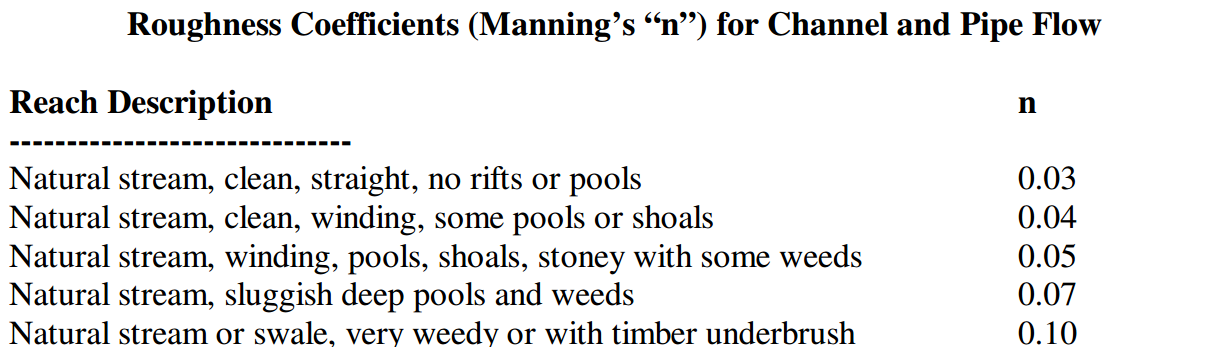
\includegraphics[keepaspectratio, width=.8\textwidth]{n_vals.png}
\caption{Commonly accepted Manning's $n$ values \cite{roughnesstable}}
\end{table}

The HAND methodology determines a height value for each 10m x 10m raster grid-cell based on that cell's nearest stream reach, determined by following the path of steepest descent using a 10m x 10m Digital Elevation Model (DEM). The HAND raster then represents the stage height requirement for each grid-cell to become inundated. For example, a HAND value of 20 ft means that the grid-cell in question is 20 ft above it's nearest stream reach, meaning that once the stream reaches a stage height of 20 ft, that particular grid-cell will become inundated. The HAND methodology is intended primarily for flood inundation mapping (ie. given a stage height, a flood extent map can be produced by showing which grid-cells are inundated), but by using an assumed maximum depth, the HAND method can also be used to approximate $A_w$ and $H_R$ for each depth interval as follows: 

\begin{description}
  \item[\bm{$A_w$}] Calculated for each assumed stage height (ie. depth interval) and a channel width measured as $(inundated grid-cells)*(grid-cell width)$.
  \item[\bm{$H_R$}] Calculated by adding the channel top-width plus the channel side-length, where top-width is calculated using total flood surface-area divided by river length, and channel side-length is calculated using the triangular geometry of each depth interval. Channels are assumed to have a trapezoidal geometry. 
\end{description}

Once all these parameters are collected, a discharge is calculated for each of the assumed stage heights, resulting in a rating curve for every stream reach in the nation. However, the accuracy of these rating curves is questionable due to DEM imperfections: DEMs are generally constructed with the use of remote sensing technologies, which frequently fail to penetrate through water surfaces. This failure to penetrate means that, at the time a land surface is remotely sensed, the lowest elevations for stream reaches will actually represent the stage height at that instant, rather than the stream's bathymetry (bottom-depth). Because of this discrepancy, and because the national HAND raster is created using the National Elevation Dataset (NED) -- which is a 10m x 10m DEM -- $A_w$ and $H_R$ as computed from the HAND rasters are likely incorrect. These discrepencies introduce potentially faulty error to the HAND-based rating curve creation previously described, and these errors must be resolved before accurate and timely predictive flood inundation maps can be produced. 

% \begin{figure}[h]
% \centering
% 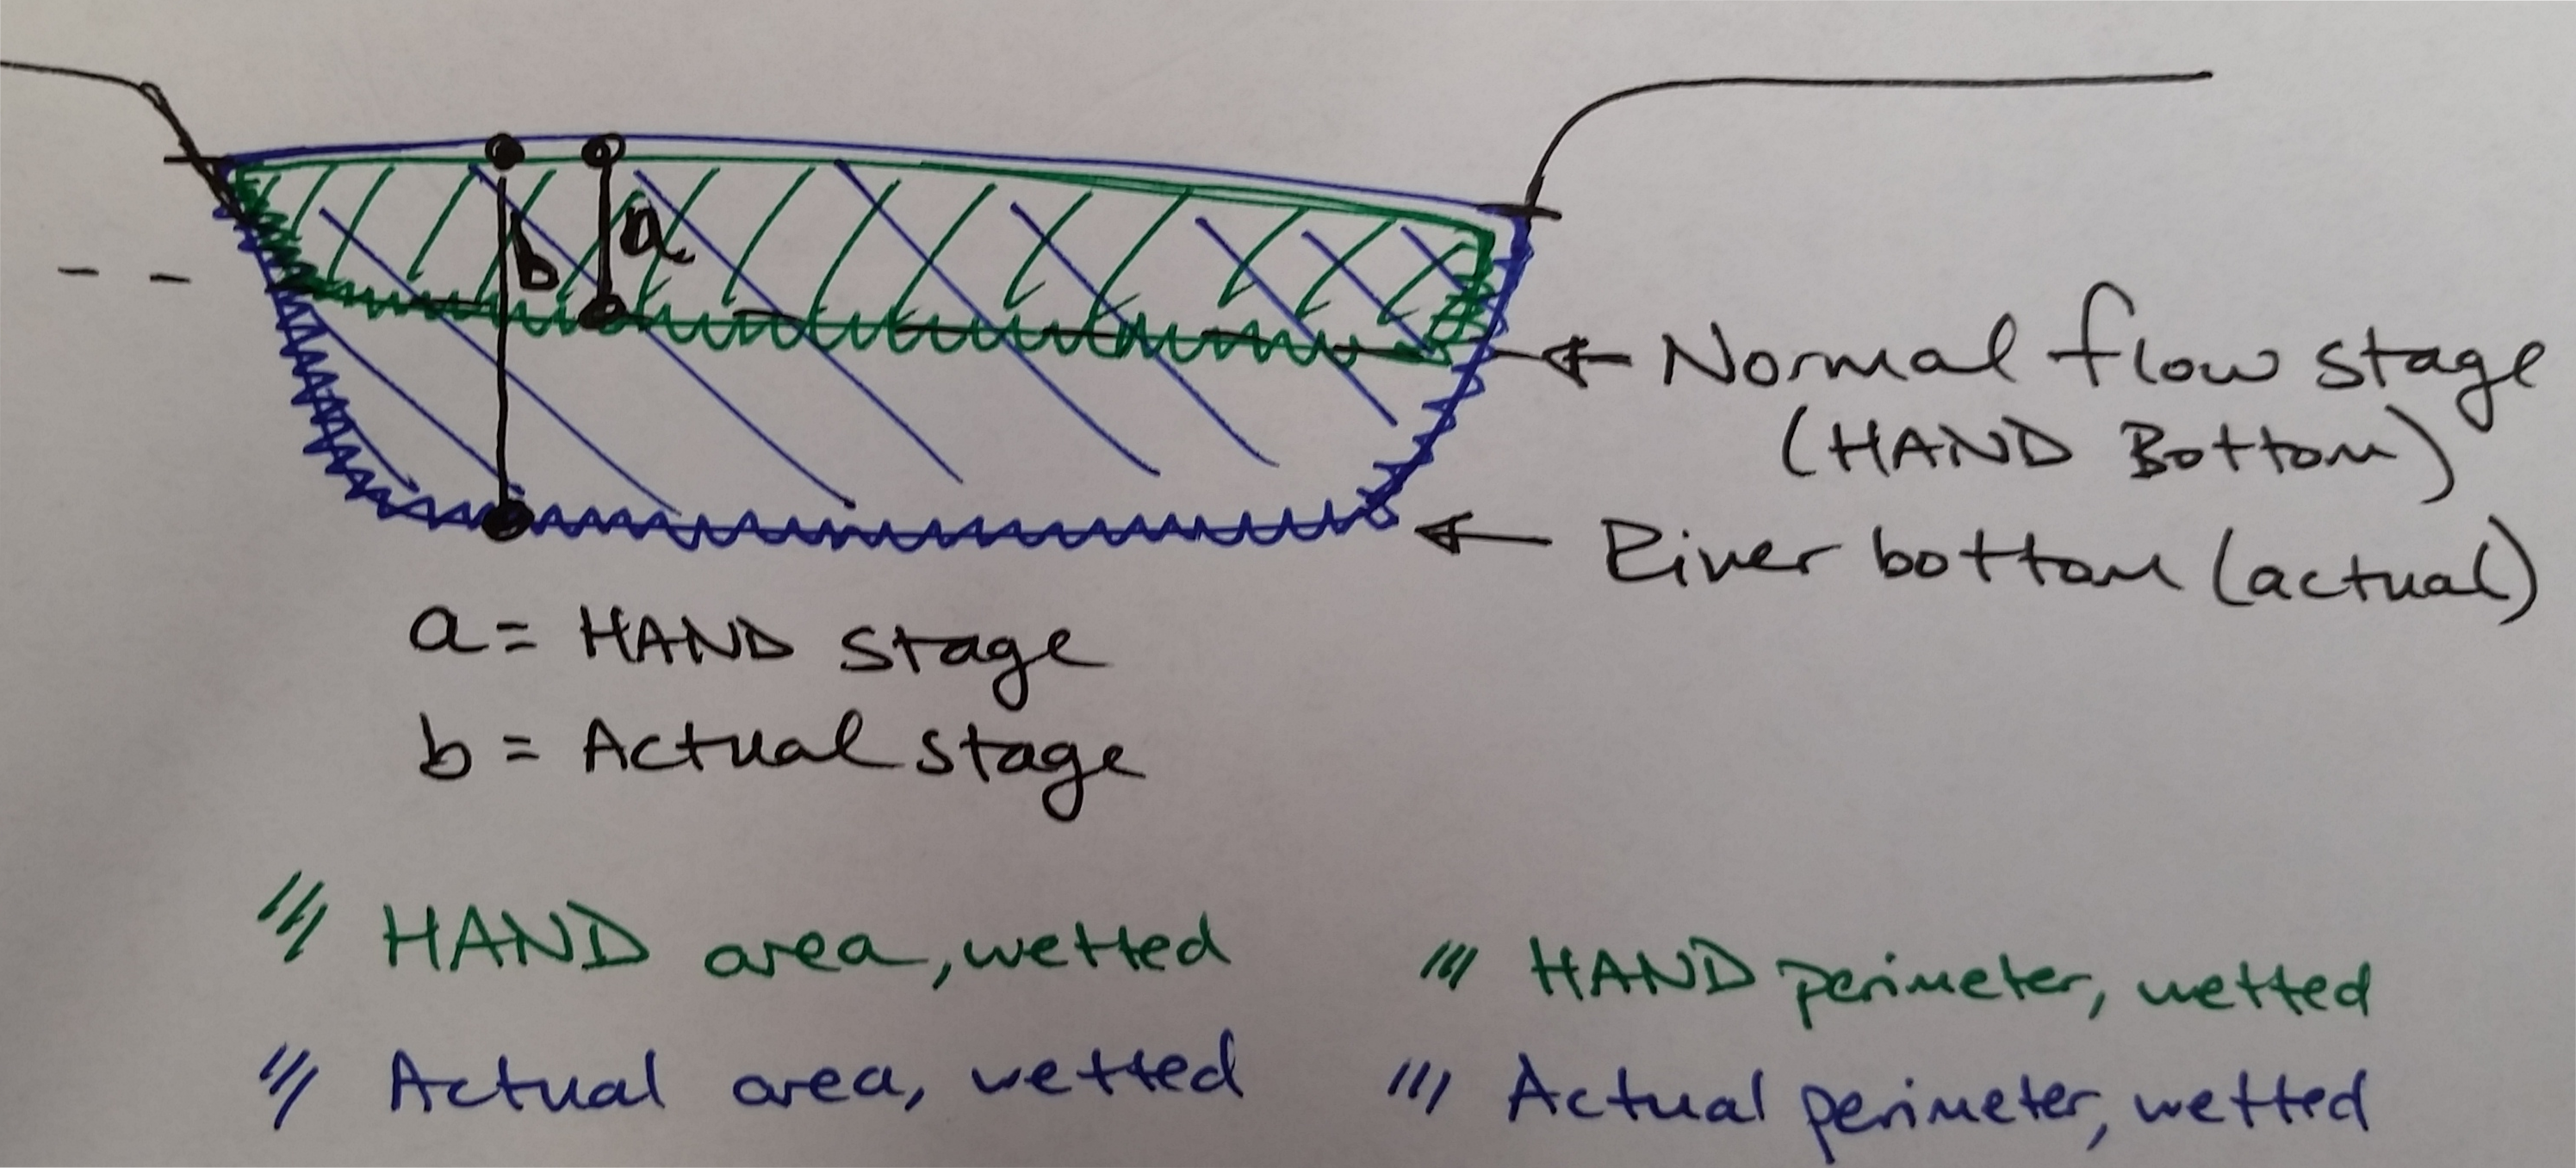
\includegraphics[keepaspectratio, width=.8\textwidth]{sketch.png}
% \caption{Sketch of variable wetted area ($A_w$) and wetted perimeter ($P_w$)} \label{fig:5}
% \end{figure}

\section*{Research Questions} % One or several research questions you want to address as part of your project.

In an effort to address the inaccuracies of HAND-based rating curves, this paper will statistically analyze how different the "theoretical" (HAND) rating curves are from the "actual" (USGS) rating curves by attempting to find a relationship between the hydraulic properties ($A_w$ and $H_R$) and other nationally-available datasets (such as the National Land Cover Dataset (NLCD)). This will be done by determining an optimal bottom-depth shift for each HAND rating curve, such that the new $A_w$ and $H_R$ generate a best-fit HAND rating curve as compared to the accepted USGS rating curve. 

\section*{Hypotheses} % Formulate a research hypothesis for each of the research questions to be tested as part of your analysis. 

The expectation is that there will be a statistically-significant relationship between the bottom-depth shifts and some nationally-available dataset, whether it be the NWM, NLCD, NED, or some other dataset.  

\section*{Literature Review} % This review can be brief, but you should provide information on the findings from previous researches such that the novelty of your work can be assessed. 

The HAND concept has been around for a while but has only recently been applied to large-scale terrain models \cite{handpaper} and flood modeling \cite{nfiehand}, and the NWM has only very recently been released (August, 2016) \cite{nwmsummary}. Regarding approximations of the hydraulic parameters involved in Manning's equation, a fair amount of research has been undertaken in the area of "At-a-station Hydraulic Geometry" and the power-law rating curve relationship (which attempt to generalize the determination of hydraulic properties for un-gaged stream reaches) \cite{ahgdingman, ahgchen}. Other research has attempted to determine hydraulic parameters using satellite measurements and hydrologic models \cite{sathydroparams}, and further research has worked to relate nationally-available datasets to Manning's $n$ for local flood modeling \cite{ahgmoore}. That said, there has been very little -- if any -- work in the area of rating curve optimization using the relatively simple and accessible statistical approach here described. 

\section*{Plan of Work} % Explain your plan of work to address the above research questions and to test your hypotheses. 

  \subsection*{Data Sets} % A concise and complete description of the data used for the analysis.

  As mentioned in the introduction, the data needed for the construction of a HAND rating curve are as follows: 

  \begin{description}
    \item[\bm{$A_w$}] Calculated using stage height and channel width.
    \item[\bm{$H_R$}] Calculated using channel top-width and channel side-length, assuming a trapezoidal channel geometry. 
    \item[\bm{$S_0$}] Retrieved from the NHDPlusV2 dataset using stream reach COMIDs \cite{nhdplusv2}.
    \item[\bm{$n$}] Assumed as 0.05 for this study, based on commonly accepted values (see Table 1).
  \end{description}

  These HAND rating curve parameters were retrieved directly from a NetCDF file containing all HAND data for Onion Creek (provided by Xing Zheng, the creator of the national HAND raster), and a HAND rating curve with no bottom-depth shift was also provided as a benchmark for assessing potential improvements. USGS rating curves can be retrieved from the USGS Water Watch Customized Rating Curve Builder for any USGS-gaged stream \cite{usgswaterwatch}. Lastly, HEC-RAS cross-sections and their associated Manning's roughness ($n$) may be retrieved for the Onion Creek watershed from Xing Zheng's masters thesis if a comparison to detailed stream reach cross-sections is needed \cite{xingms}.

  \subsection*{Methods} % Which methods you will be using in your analysis. 

  The intended approach will be to first select a single stream reach in the Onion Creek watershed in Austin, Texas, and to manually increase the bottom-depth shift by an incremental value (effectively changing the HAND cross-section). At each incremental step, a new $A_w$ and $H_R$ can be calculated for each 1-foot depth interval, effectively creating a new HAND-based rating curve. This new HAND rating curve will then be plotted against the respective USGS rating curve, and a root-mean-square-error (RMSE) will be calculated. In a similar way, many HAND-based rating curves will be programatically calculated for the stream reach in question for varying bottom-depth shifts, and by minimizing the RMSE, an optimal bottom-depth shift will be determined for that reach. 

  \subsection*{Preliminary Results} % What you have obtained so far.

  Rating curves have already been programatically created for all USGS-gaged streams in the Onion Creek watershed, and the USGS rating curves have been manually shifted downwards to assign a discharge of 0.01 cfs to a bottom-depth of 0 feet. Relevant HAND rating curves have also been both manually and programatically snapped to these adjusted USGS rating curves by tweaking the roughness coefficient, though adjustments to the roughness coefficient have since been decided to be inappropriate, seeing as Manning's roughness values describe physical stream characteristics and should therefore not be altered. An example of a rating curve fitting using manual snapping (manually altering Manning's $n$ to visually fit the rating curves) and automatic snapping (back-calculating Manning's $n$ for each available 1-foot interval in a shifted USGS rating curve, averaging all Manning's $n$ values for that stream reach, then applying the average $n$ to the HAND rating curve) is shown here for detail (see figure 2). 

  \begin{figure}[h]
  \makebox[\linewidth][c]{
  \begin{subfigure}{0.6\textwidth}
    \centering
    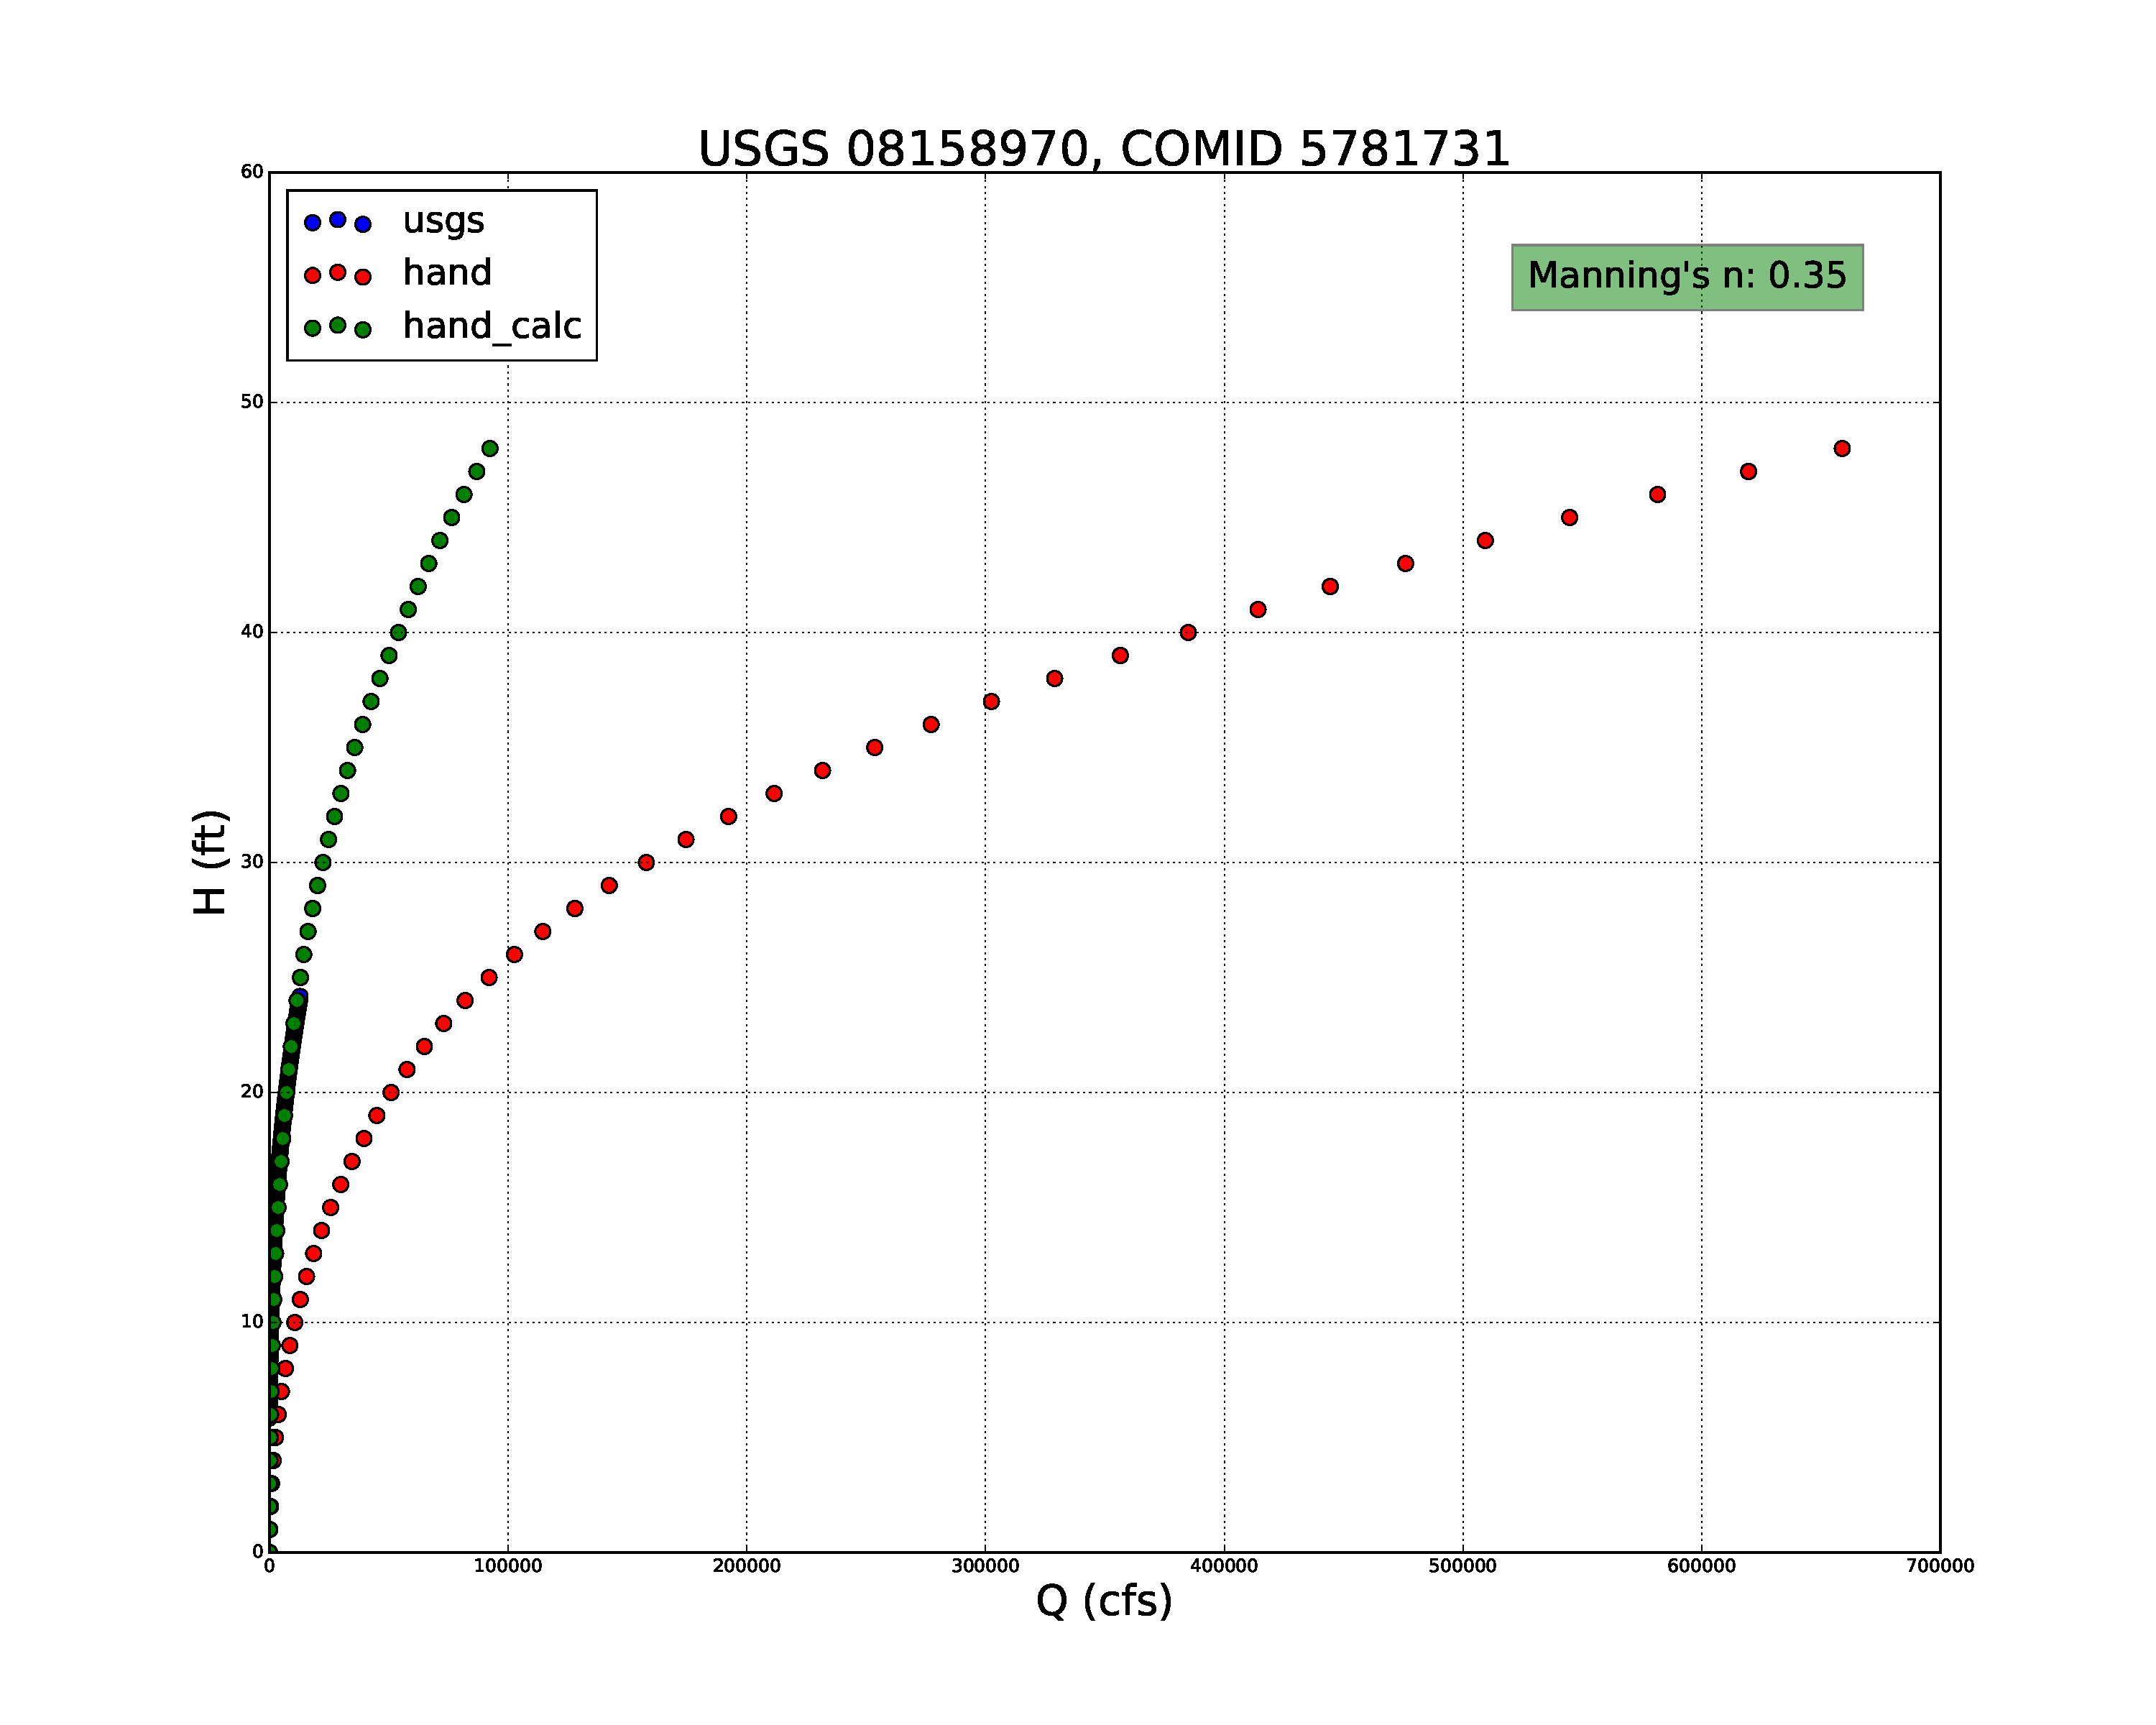
\includegraphics[width=\linewidth]{5781731_manual.pdf}
    \caption{Manually-Adjusted Rating Curve}\label{fig:a}
  \end{subfigure}\hspace*{\fill}
  \begin{subfigure}{0.6\textwidth}
    \centering
    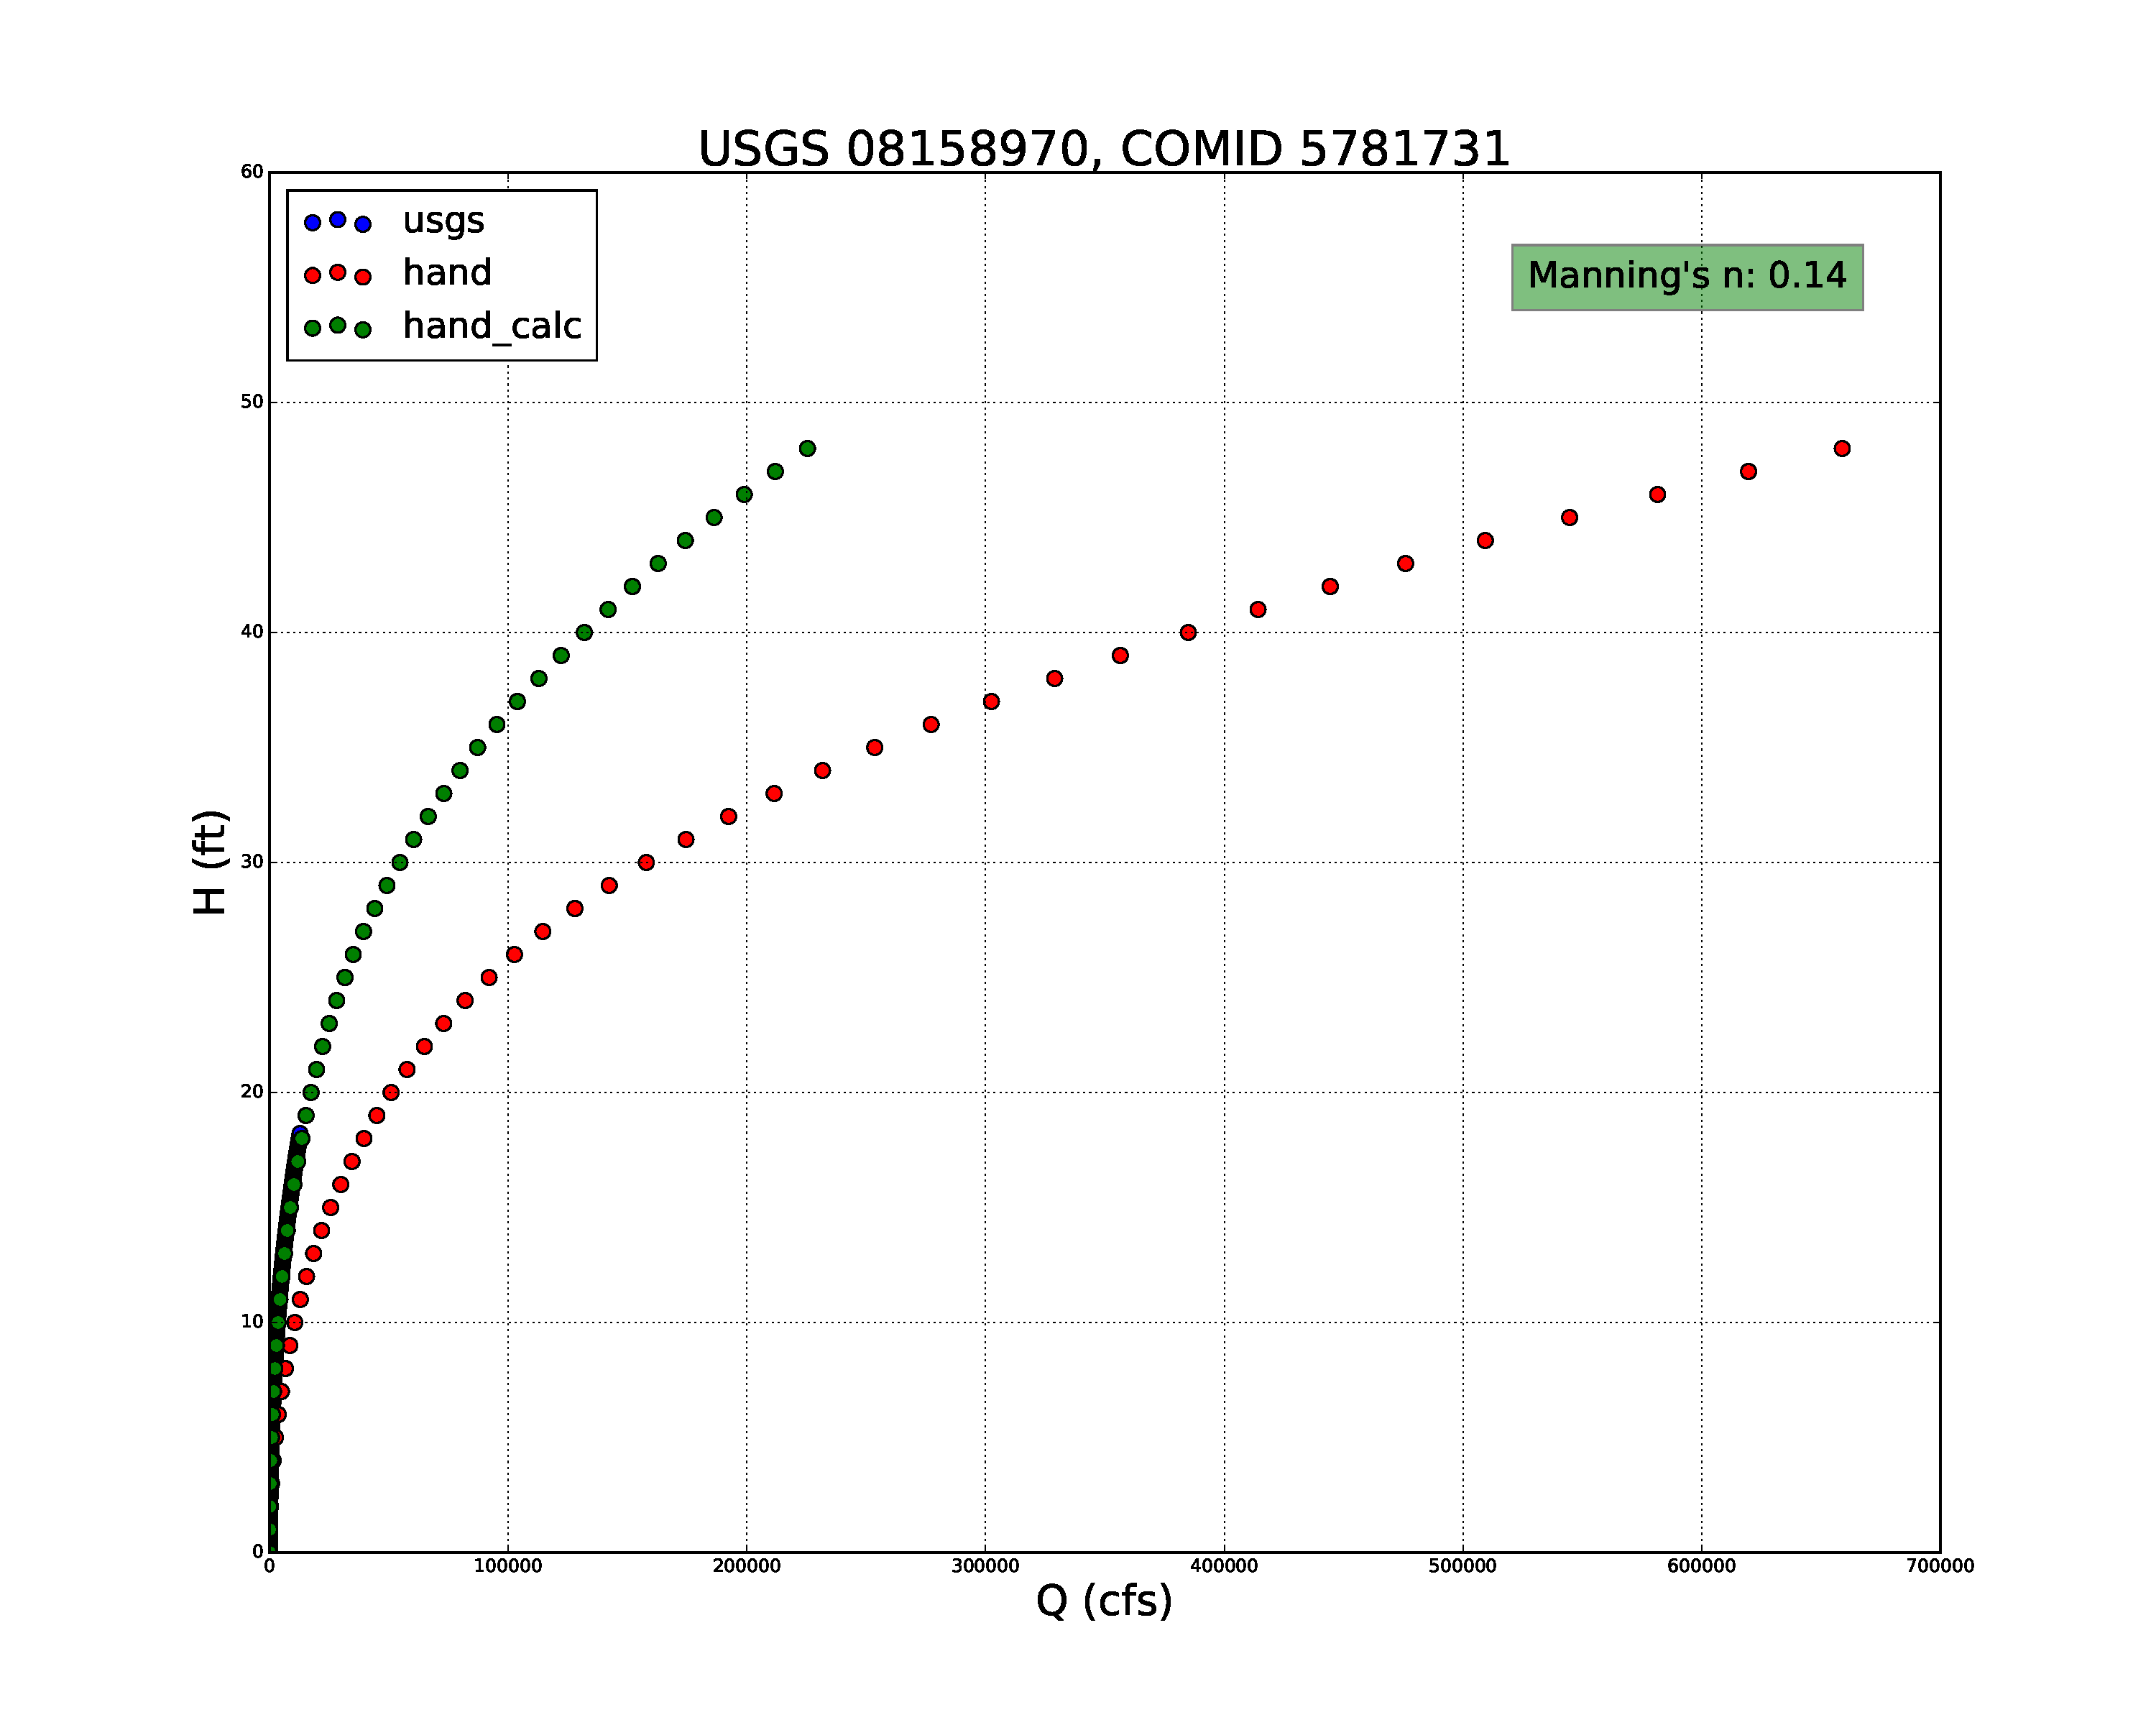
\includegraphics[width=\linewidth]{5781731_auto.pdf}
    \caption{Automatically-Adjusted Rating Curve}\label{fig:b}
  \end{subfigure}\hspace*{\fill}
  }
  \caption{Manual vs. Automatic Adjustments for COMID 5781731 Rating Curve} \label{fig:2}
  \end{figure}

  \subsection*{Future Work} % What you are planning on doing next.

  Once an optimal bottom-depth shift is determined for each stream reach containing a USGS gage, a relationship between the bottom-depth shifts and a nationally-available dataset (ie. NWM, NLCD, or NED) will be sought using a two-parameter statistical test. An additional test may be run to assess the "correctness" of the new bottom-depth shift by comparing the shifted HAND cross-sections with "actual" HEC-RAS cross-sections. This HEC-RAS cross-sectional data has already been compiled for the Onion Creek watershed, making this a fairly simple comparison. \cite{xingms}. 

  This relationship will be computationally tested by ideally implementing a machine-learning algorithm applied on a small subset of stream reaches with USGS gages, validated on the remaining USGS-gaged streams, and finally extended to approximate the bottom-depth shifts necessary for all remaining $\sim$2.7 million stream reaches in the nation.

\printbibliography

\end{document}

% \begin{quote}
% \small
% The [NWM] runs an hourly uncoupled analysis (simulation of current conditions). Short-range forecasts are executed hourly while medium-range forecasts out to 10 days are produced once per day. A daily ensemble long range forecast to 30-days is also produced. All model configurations provide streamflow for 2.7 million river reaches and other hydrologic information on 1km and 250m grids. \cite{nwmsummary}
% \end{quote}

% \noindent